%!TEX root = ../Main.tex

% -----------------------------------------------------------------------------
\section{Processes, Machines, Combinators and Operators}
\label{s:Processes}

A \emph{process} in our system is a simple imperative program with a local heap. A process pulls data from an arbitrary number of input streams and pushes result values to at least one output stream. The process language is an intermediate representation we use when fusing the overall dataflow network. When describing the fusion transform we describe the control flow of the process as a state machine, hence Machine Fusion. 

A \emph{combinator} is a template for a particular process which parameterises it over the particular input and output streams, as well as values of configuration parameters such as the worker function used in a @map@ process. Each process implements a logical \emph{operator} --- so we use ``operator'' when describing the values being computed, but ``process'' and ``machine'' when referring to the implementation. 


% -----------------------------------------------------------------------------
\subsection{Grouping}

The definition of the @group@ combinator which removes consecutive elements from its input stream is given in Fig.~\ref{fig:Process:Group}. We include the concrete code representation and a diagram of the process viewed as a state machine.

The @group@ combinator has two parameters, @sIn1@ and @sOut1@, which bind the input and output streams respectively. The \emph{nu-binders} \mbox{$\nu$ @(f: Bool) (l: Nat)@...} indicate that each time the @group@ combinator is instantiated, fresh names must be given to @f@, @l@ and so on, that do not conflict with other instantiations. 

The body of the combinator is a record that defines the process. The @ins@ field of the record defines the set of input streams and the @outs@ field the set of output streams. The @heap@ field gives the initial values of each of the local variables. The @instrs@ field contains a set of labeled instructions that define the program, while the @label@ field gives the label of the initial instruction. 

%%% AR: Should we explain intuition behind how process works and @f@, @l@, @v@ before detailed instructions?

The initial instruction @(pull sIn1 v A1 [])@ pulls the next element from the stream @sIn1@, writes it into the heap variable @v@ (value), then proceeds to the instruction at label @A1@. The empty list @[]@ after the target label @A1@ can be used to update heap variables, but as we do not need to update anything yet we leave it empty. 

Next, the instruction @(case (f || (l /= v)) A2 [] A3 [])@ checks whether predicate @(f || (l /= v))@ is true; if so it proceeds to the instruction at label @A2@, otherwise it proceeds to @A3@. We use the variable @l@ (last) to track the last value read from the stream, and the boolean @f@ (first) for whether this is the first element.

When the predicate is true, the instruction @(push sOut1 v A3 [ l = v, f = F ])@ pushes the value @v@ to the output stream @sOut1@ and proceeds to the instruction at label @A3@, once the heap has been updated to set variable @l@ to @v@ and @f@ to @F@ (False). 

Finally, the instruction @(drop sIn1 A0 [])@ signals that the current element that was pulled from stream @sIn1@ is no longer required, and goes back to the first the instruction at @A0@. This @drop@ instruction is used to coordinate concurrent processes when performing fusion. The next element of a stream may only be pulled after all consumers have pulled and then and dropped the current element.

Overall, the @f@ variable tracks whether we are dealing with the first value from the stream, @l@ holds the last value pulled from the stream (or 0 if none have been read yet), and @v@ holds the current value pulled from the stream. The process emits the first value pulled from the stream and every value that is different from the last one that was pulled. For example, when executed on the input stream $[1, 2, 2, 3]$, the process will produce the output $[1, 2, 3]$.

\begin{figure}

\begin{center}
\begin{alltt}
           group 
             = \(\lambda\) (sIn1: Stream Nat) (sOut1: Stream Nat). 
               \(\nu\) (f: Bool) (l: Nat) (v: Nat) (A0..A3: Label).
\end{alltt}
\begin{code}
               process
               { ins:    { sIn1  }
               , outs:   { sOut1 }
               , heap:   { f = T, l = 0, v = 0 }
               , label:  A0
               , instrs: { A0 = pull sIn1 v          A1 []
                         , A1 = case (f || (l /= v)) A2 []  A3 []
                         , A2 = push sOut1 v         A3 [ l = v, f = F ]
                         , A3 = drop sIn1            A0 [] } }
\end{code}
\end{center}
\vspace{1em}
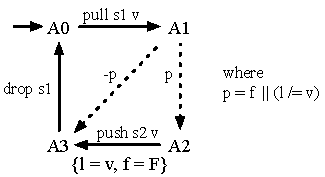
\includegraphics[scale=1.1]{figures/state-group.pdf}
\caption{The group combinator}
\label{fig:Process:Group}
\end{figure}


% -----------------------------------------------------------------------------
\subsection{Merging}
\begin{figure}
\begin{alltt}
               merge
                 = \(\lambda\) (sIn1: Stream Nat) (sIn2: Stream Nat) (sOut2: Stream Nat). 
                   \(\nu\) (x1: Nat) (x2: Nat) (B0..E2: Label).
\end{alltt}
\begin{code}
                   process
                   { ins:    { sM1, sM2 }
                   , outs:   { sM3 }
                   , heap:   { x1 = 0, x2 = 0 }
                   , label:  B0
                   , instrs: { B0 = pull sIn1  x1   B1 []
                             , B1 = pull sIn2  x2   C0 []
                             , C0 = case (x1 < x2)  D0 []  E0 []
                             , D0 = push sOut2 x1   D1 []
                             , D1 = drop sIn1       D2 []
                             , D2 = pull sIn1  x1   C0 []
                             , E0 = push sOut2 x2   E1 []
                             , E1 = drop sIn2       E2 []
                             , E2 = pull sIn2 x2    C0 [] } }
\end{code}

\medskip
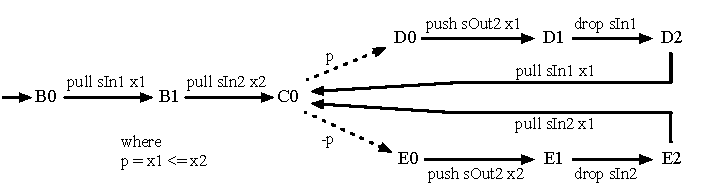
\includegraphics[scale=1.1]{figures/state-merge.pdf}
\caption{The merge combinator}
\label{fig:Process:Merge}
\end{figure}

The definition of the @merge@ combinator, which merges two input streams, is given in Fig.~\ref{fig:Process:Merge}. The combinator binds the two input streams to @sIn1@ and @sIn2@, while the output stream is @sOut2@. The two heap variables @x1@ and @x2@ are used to store the last values read from each input stream. The process starts by pulling from each of the input streams. It then compares the two pulled values, and pushes the smaller of the values to the output stream. The process then drops the stream which yielded the the smaller value, then pulls from the same stream so that it can perform the comparison again.

As this the @merge@ process merges infinite streams, if we execute it with a finite input prefix, it will arrive at an intermediate state that may not yet have pushed all available output. For example, if we execute the process with the input streams $[1, 4]$ and $[2, 3, 100]$ then the values $[1, 2, 3, 4]$ will be pushed to the output. After pushing the last value $4$, the process will block at instruction @E2@, waiting for the next value to become available from @sIn2@. We discuss how to handle finite streams later in ~\S\ref{s:Finite}.


% -----------------------------------------------------------------------------
\subsection{Fusion}

Our fusion algorithm takes two process state machines and produces a new one that computes the outputs of both. For example, suppose we need a single machine that computes the outputs of the first two combinators of our @uniquesUnion@ example back in \S\ref{s:Introduction}. The result will be a machine that computes the result of both the @group@ and @merge@ as if they were executed concurrently, where the first input stream of the @merge@ is the same as the input stream of the @group@. For ease of comparison we will assume the parameters in each combinator are instantiated by arguments with the same names.


% -----------------------------------------------------------------------------
\subsubsection{Fusing Pulls}
\label{s:Fusion:FusingPulls}

The algorithm proceeds by considering pairs of states: one in each of the machines to be fused. Both the @group@ machine and the @merge@ machine pull from the same stream as their initial instruction, so we have the situation shown in Fig.~\ref{fig:Fusion:Pulls}. The @group@ machine needs to transition from label @A0@ to label @A1@, and the @merge@ machine from @B0@ to @B1@. In the result machine we produce three new instructions that transition between four result states, @F0@ to @F3@.
Each of the result states represents a combination of two original states, one from each of the input machines. For example, the first result state @F0@ represents a combination of the @group@ machine being in its initial state @A0@ and the @merge@ machine being in its own initial state @B0@. 

We also associate each of the result states with information describing whether or not each machine has already pulled a value from each input stream. For the @F0@ case shown in Fig.~\ref{fig:Fusion:Pulls} we have ((A0, \{sIn1 = none\}), (B0, \{sIn1 = none, sIn2 = none\})). The result state @F0@ represents a combination of the two input states @A0@ and @B0@. As both @A0@ and @B0@ are the initial states of their respective machines, those machines have not yet pulled any values from their two input streams, so both `sIn1' and `sIn2' map to `none'.

From the joint state @F0@, both of the input machines then need to pull from stream @sIn1@, the @group@ machine storing the value in a variable @v@ and the @merge@ machine storing it in @x1@. In the result machine this is managed by first storing the pulled value in a fresh buffer variable @b1@, and then using later instructions to copy the value into the original variables @v@ and @x1@. For this we attach updates to a @jump@ instruction, which otherwise transitions between states without affecting any of the input or output streams.

Finally, note that in the result states @F0@ through @F3@ the state of the input streams transition from `none', to `pending' then to `have'. The `none' state means that we have not yet pulled a value from the associated stream. The `pending' state means we have pulled a value into the stream buffer variable (@b1@ in this case). The `have' state means that we have copied the pulled value from the stream buffer variable into the local variable used by each machine. In Fig.~\ref{fig:Fusion:Pulls},  `sIn1' is set to `have' for the first machine in @F2@ after we have set `v = b1', while `sIn1' is set to `have' for the second machine in @F3@ after we have set `x1 = b1'. 


\begin{figure}
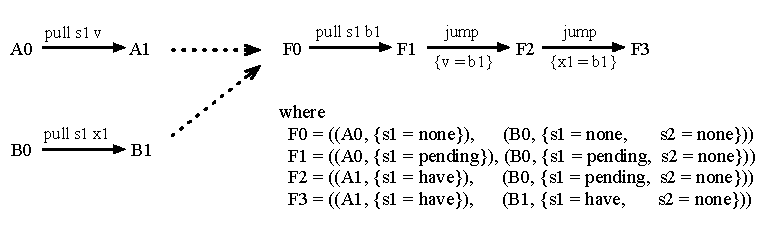
\includegraphics[scale=1.1]{figures/fuse-pull-pull.pdf}
\caption{Fusing pull instructions}
\label{fig:Fusion:Pulls}
\end{figure}


% -----------------------------------------------------------------------------
\subsubsection{Fusing Cases}
\begin{figure}
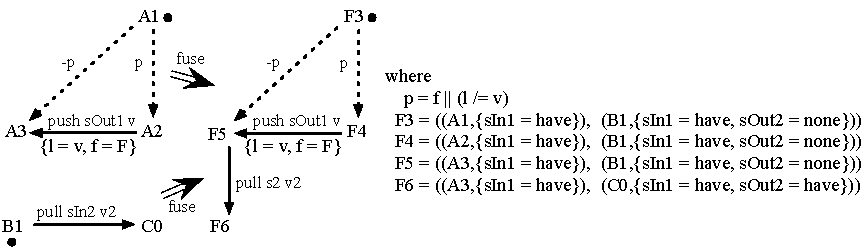
\includegraphics[scale=1.1]{figures/fuse-case-pull.pdf}
\caption{Fusing case instructions}
\label{fig:Fusion:Case}
\end{figure}

Once the result machine has arrived in the joint state @F3@, this is equivalent to the two input machines arriving in states @A1@ and @B1@ respectively. The left of Fig.~\ref{fig:Fusion:Case} shows the next few transitions of these machines. From state @A1@, the @group@ machine needs to perform a @case@ branch to determine whether to push the current value it has from its input stream @sIn1@ to its output stream @sOut1@, or to just move on to the next value from its input. From state @B1@, the @merge@ machine needs to pull a value from its second input stream @sIn2@. In the result machine, @F3@ performs the case analysis from @A1@, moving to either @A2@ or @A3@, corresponding to @F4@ and @F5@ respectively. At @F4@, the push at @A2@ is executed and moves to @A3@, corresponding to @F5@.

Finally, at @F5@ the @merge@ machine pulls from @sIn2@, moving from @B1@ to @C0@.
Because the stream @sIn2@ is only pulled from by the @merge@ machine, no coordination is required between @merge@ and @group@ for this pull.

Note that we could construct the fused result machine in several ways. One option is to perform the case branch first and then pull from @sIn2@, another is to pull from @sIn2@ first and then perform the branch. By construction, the predicate used in the branch refers only to variables local to the @group@ machine, and the pull instruction from @B1@ stores its result in a variable local to the @merge@ machine. As the set of variables does not overlap, either ordering is correct. For this example we choose to perform the branch first, though will discuss the ramifications of this choice further in \S\ref{s:FusionOrder}. 


% -----------------------------------------------------------------------------
\subsection{Fused Result}

Fig.~\ref{fig:Process:Fused} shows the end result of fusing @group@ and @merge@ together. There are other rules for handling different combinations of instructions, but we defer the details to \S\ref{s:Fusion}. The result process has two inputs, @sIn1@ and @sIn2@, which correspond to the original input streams. It also has two outputs, @sOut1@ which is the @group@ processes output stream, while @sOut2@ is the @merge@ processes output stream. 

Overall, our fusion algorithm has taken two separate processes that we once imagined to be running concurrently, and has produced a single sequental result process that implements both. We have chosen a \emph{specific sequential order} in which to interleave instructions that implement both original processes. As with the Flow Fusion system of \citet{lippmeier2013data} we have performed the job of a concurrent scheduler at compile time. However, in contrast to Flow Fusion and similar systems, we do not need to organize statements into a fixed \emph{loop anatomy}, we simply merge them as they are. This allows us to implement a wider range of processes, including ones with nested loops that work on segmented streams, which we discuss further in \S\ref{s:FutureWork}. 

To complete the implementation of our example from \S\ref{s:Introduction} we would now proceed to fuse the process from the final line (also a @group@) into this new result process. The order in which processes are fused together does matter, as does the order in which the instructions are emitted --- we discuss both points further in \S\ref{s:Evaluation}.

Finally, although the result process has a single shared heap, the bindings are guaranteed not to interfere. When we instantiated combinators to create the original processes we introduced fresh names at that point. The stream buffer variables we aditionally introduced for coordination were freshly created during fusion.

%%% AR: would like to highlight which machine is performing the current instruction, eg bolding "A0" when it's group moving from A0 to A1
\begin{figure}
\begin{code}
process
{ ins:    { sIn1,  sIn2 }
, outs:   { sOut1, sOut2 }
, heap:   { f = T, l = 0, v = 0, x1 = 0, x2 = 0, b1 = 0}
, label:  F0
\end{code}

\definecolor{groupc}{HTML}{308030}
\definecolor{mergec}{HTML}{800000}
\definecolor{sharec}{HTML}{000080}

\newcommand\annot[5]{
  \tiny ((#1,   \> \tiny \{sIn1 =      #2\}), 
                \> \tiny (#3, \> \tiny \{sIn1 =      #4, \> \tiny sIn2 =      #5\}))
}

\newcommand\icase[7]{
 \tt{#1} \> \tt{= #2} \> \tt{#3} \> \tt{[ #4 ]} \> \tt{#5} \> \tt{[ #6 ]} \> \tiny #1 \> \tiny = #7
}
\newcommand\instr[5]{
 \tt{#1}\>\tt{= #2} \> \tt{#3} \> \tt{[ #4 ]} \> \> \> \tiny #1 \> \tiny = #5
}

\begin{tabbing}
@  @ \=
@, F17@  \= = @case (f || (l /= v)) @
         \= @F17@ \= @[ ]     @ \= @F17@ \= @[ ]@
@   @ \= \tiny @   @F17 \= \tiny = ((A0, \= \tiny \{sIn1 = pending\}), \= \tiny (B0, \= \tiny \{sIn1 = pending, \= \tiny sIn2 = pending\})) \kill

@, instrs:@

% I have no idea how this works, but you need this particular incantation to colour the whole line in a tabbing environment.
% It's not ideal that the { and , are coloured too, but that can't be helped.
\\[0pt \color{sharec}]
\> @{@
\instr{F0}{pull sIn1 b1}{F1}{}
      {\annot{A0}{none}{B0}{none}{none}}

\\[0pt \color{groupc}]
\> @,@
\instr{F1}{jump}{F2}{v  = b1}
      {\annot{A0}{pending}{B0}{pending}{none}}

\\[0pt \color{mergec}]
\> @,@
\instr{F2}{jump}{F3}{x1 = b1}
      {\annot{A1}{have}{B0}{pending}{none}}

\\[0pt \color{groupc}]
\> @,@
\icase{F3}{case (f || (l /= v))}{F4}{}{F5}{}
      {\annot{A1}{have}{B1}{have}{none}}

\\[0pt \color{groupc}]
\> @,@
\instr{F4}{push sOut1 v}{F5}{l = v, f = F}
      {\annot{A2}{have}{B1}{have}{none}}

\\[0pt \color{groupc}]
\> @,@
\instr{F5}{jump}{F6}{}
      {\annot{A3}{have}{B1}{have}{none}}

\\[0pt \color{mergec}]
\> @,@
\instr{F6}{pull sIn2 x2}{F7}{}
      {\annot{A0}{none}{B1}{have}{none}}

\\
\\[0pt \color{mergec}]
\> @,@
\icase{F7}{case (x1 < x2)}{F8}{}{F16}{}
      {\annot{A0}{none}{C0}{have}{have}}

\\
\\[0pt \color{mergec}]
\> @,@
\instr{F8}{push sOut2 x1}{F9}{}
      {\annot{A0}{none}{D0}{have}{have}}

\\[0pt \color{mergec}]
\> @,@
\instr{F9}{drop sIn1}{F10}{}
      {\annot{A0}{none}{D1}{none}{have}}

\\[0pt \color{sharec}]
\> @,@
\instr{F10}{pull sIn1 b1}{F11}{}
      {\annot{A0}{none}{D2}{none}{have}}

\\[0pt \color{groupc}]
\> @,@
\instr{F11}{jump}{F12}{v = b1}
      {\annot{A0}{pending}{D2}{pending}{have}}

\\[0pt \color{mergec}]
\> @,@
\instr{F12}{jump}{F13}{x1 = b1}
      {\annot{A1}{have}{D2}{pending}{have}}

\\[0pt \color{groupc}]
\> @,@
\icase{F13}{case (f || (l /= v))}{F14}{}{F15}{}
      {\annot{A1}{have}{C0}{have}{have}}

\\[0pt \color{groupc}]
\> @,@
\instr{F14}{push sOut1 v}{F15}{l = v, f = F}
      {\annot{A2}{have}{C0}{have}{have}}

\\[0pt \color{groupc}]
\> @,@
\instr{F15}{jump}{F7}{}
      {\annot{A3}{have}{C0}{have}{have}}

\\

\\[0pt \color{mergec}]
\> @,@
\instr{F16}{push sOut2 x2}{F17}{}
      {\annot{A0}{none}{E0}{have}{have}}

\\[0pt \color{mergec}]
\> @,@
\instr{F17}{drop sIn2}{F18}{}
      {\annot{A0}{none}{E1}{have}{have}}

\\[0pt \color{mergec}]
\> @,@
\instr{F18}{pull sIn2}{F7}{}
      {\annot{A0}{none}{E2}{have}{none}}


\\[0pt \color{black}]
@} }@
\end{tabbing}

\caption{Fusion of group and merge}
\label{fig:Process:Fused}
\end{figure}


% -----------------------------------------------------------------------------
% BL: This is too much low level detail at this point, we need more intuition.

% The instructions of @merge@ can be split into four categories, which can be identified in the fused process: labels @B0@-@B2@ perform initialisation, and are mapped to @F0@-@F6@; label @C0@ performs case analysis to find the smaller value and is mapped to @F7@; labels @D0@-@D2@ push the value from the first stream, @s1@, and are mapped to @F8@-@F15@; and labels @E0@-@E2@ push the value from the second stream, @s2@, and are mapped to @F16@-@F18@.

% The @group@ process can also be identified in the fused process: the fused labels @F0@-@F5@ perform the pulling, case analysis and pushing from instructions @A0@-@A2@. These instructions are seen again in @F10@-@F14@, when the @merge@ process is pulling from the @s1@ stream. Thus the @group@ instructions have been duplicated, and are performed once when @merge@ initialises, and again every time @merge@ pulls from the first stream.

% Labels @F5@ and @F14@ correspond to the (@drop s1@) instruction at @A3@ in @group@, but note that they are fused as @jump@ instructions. As @s1@ is shared between the two processes, the element from @s1@ can only be dropped once both processes agree to drop. In the fused labels on the right hand column, the other process still has @s1@ as `pending' or `have', so the element cannot yet be dropped. The actual @drop@ is only performed once both processes are `none', at label @F9@.
 
